% Demo report: sending embeddings from 10 edge nodes to one node with NebulaStream.
% Build:  python reports/make_report.py   (regenerates the figures and numbers.tex from output/results.csv)
%         cd reports && latexmk -pdf demo_report.tex
\documentclass[11pt,a4paper]{article}

\usepackage[T1]{fontenc}
\usepackage[utf8]{inputenc}
\usepackage{lmodern}
\usepackage[margin=2.2cm]{geometry}
\usepackage{graphicx}
\usepackage{booktabs}
\usepackage{float}  % [H]: keep figures under their section
\usepackage{caption}
\usepackage{xcolor}
\usepackage[hidelinks]{hyperref}

\captionsetup{font=small,labelfont=bf}
\setlength{\parskip}{4pt}
\setlength{\parindent}{0pt}

% GENERATED by reports/make_report.py from output/results.csv -- do not edit
\newcommand{\nWorkers}{10}
\newcommand{\rowsPerWorker}{200}
\newcommand{\rowsTotal}{2{,}000}
\newcommand{\rowsExpected}{2{,}000}
\newcommand{\dims}{32}
\newcommand{\rowBytes}{144}
\newcommand{\refGroup}{sci.space}
\newcommand{\embKB}{281}
\newcommand{\rawKB}{2{,}356}
\newcommand{\ratio}{8.4}
\newcommand{\maxEmbErr}{0}
\newcommand{\maxScoreErr}{5.7\times 10^{-7}}
\newcommand{\refMean}{+0.40}
\newcommand{\nextBest}{+0.10}
\newcommand{\nRef}{100}
\newcommand{\refInTop}{81}
\newcommand{\allDelivered}{every worker 200/200}
  % generated by make_report.py: \nWorkers, \rowsTotal, \ratio, ...

\newcommand{\code}[1]{\texttt{#1}}
\newcommand{\grp}[1]{\textit{#1}}

\title{Sending embeddings from \nWorkers{} edge nodes to one node with NebulaStream}
\author{Vasil \textperiodcentered{} Demo report, LLMs in Hierarchical Aggregation Topologies}
\date{\today}
\makeatletter\renewcommand{\@maketitle}{%
  {\LARGE\bfseries \@title\par}\vspace{4pt}
  {\@author\ \textperiodcentered{} \@date\par}\vspace{10pt}}\makeatother

\begin{document}
\maketitle

\section{What was run}

\nWorkers{} NebulaStream edge workers (A1--A\nWorkers) each read a slice of the 20~Newsgroups dataset
that was turned into sentence embeddings beforehand (\code{all-MiniLM-L6-v2}, reduced from 384 to
\dims{} dimensions with PCA and normalised to unit length). Each worker holds posts from two
newsgroups and sends \rowsPerWorker{} rows downstream to a single sink worker~B. A row is only
\code{WORKER\_ID}, \code{TS} and \dims{} \code{FLOAT32} values (\rowBytes{}~bytes); the text itself
never enters the topology.

B runs one SQL expression on every incoming row: \code{SCORE} is the cosine similarity between the
embedding and a fixed reference vector, the centroid of all \grp{\refGroup} posts. The edge workers
are configured with \code{max\_operators: 0}, so NebulaStream places this computation on~B, not at
the edge (verified in the query plan). B writes \code{WORKER\_ID}, \code{TS}, \code{SCORE} and the
embedding to a CSV file, which is the only input of both figures below.

\section{Did everything arrive?}

B's output was compared row by row with what each worker sent (Table~\ref{tab:delivery}).

\begin{table}[H]
  \centering
  \begin{tabular}{ll}
    \toprule
    Rows received at B                     & \rowsTotal{} of \rowsExpected{} (\allDelivered) \\
    Embeddings at B vs.\ as sent            & bit-identical (max.\ difference \maxEmbErr) \\
    \code{SCORE} at B vs.\ same formula in Python & max.\ difference $\maxScoreErr$ (float32 rounding) \\
    Bytes sent as embeddings               & \embKB{}~KB \\
    Same posts as raw text                 & \rawKB{}~KB, i.e.\ \ratio$\times$ more than the embeddings \\
    \bottomrule
  \end{tabular}
  \caption{Delivery check: B's output against what the \nWorkers{} edge workers sent.}
  \label{tab:delivery}
\end{table}

\section{What B received, coloured by its score}

\begin{figure}[H]
  \centering
  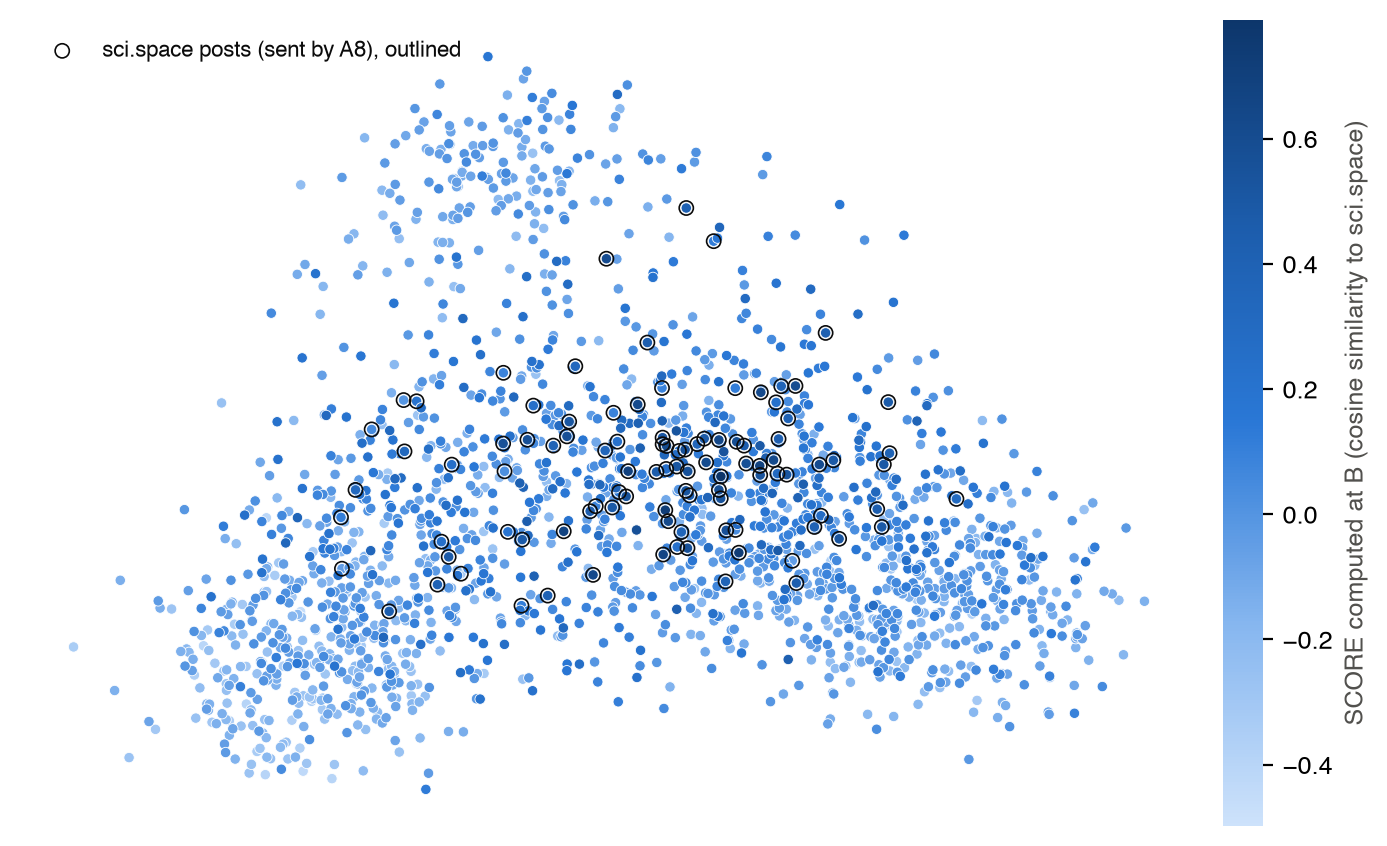
\includegraphics[width=0.9\linewidth]{fig1_projection_by_score.png}
  \caption{Every point is one of the \rowsTotal{} rows B received. The \dims-dimensional embeddings
    are projected to two dimensions with PCA (the axes have no units; only distances matter). Colour
    is the \code{SCORE} that B computed in NebulaStream. Outlined points are the \grp{\refGroup}
    posts; this label comes from the dataset and was never sent to~B.}
  \label{fig:projection}
\end{figure}

The darkest points in Figure~\ref{fig:projection}, i.e.\ the rows B scored as most similar to
\grp{\refGroup}, are not scattered randomly: they are concentrated in one part of the plot, and the
outlines show that they are mostly the \grp{\refGroup} posts sent by worker~A8. The \grp{\refGroup}
rows average a score of $\refMean$, while the next-highest of the other 19 newsgroups averages only
$\nextBest$. Of the \nRef{} \grp{\refGroup} rows, \refInTop{} are among the 200 highest-scoring rows
(top 10\,\%). B never saw any text, only \dims{} numbers per post, yet its computation recognises the
topic. The embeddings therefore kept their meaning after travelling from the edge nodes through the
topology to~B.

\section{Each node's data stays recognisable}

\begin{figure}[H]
  \centering
  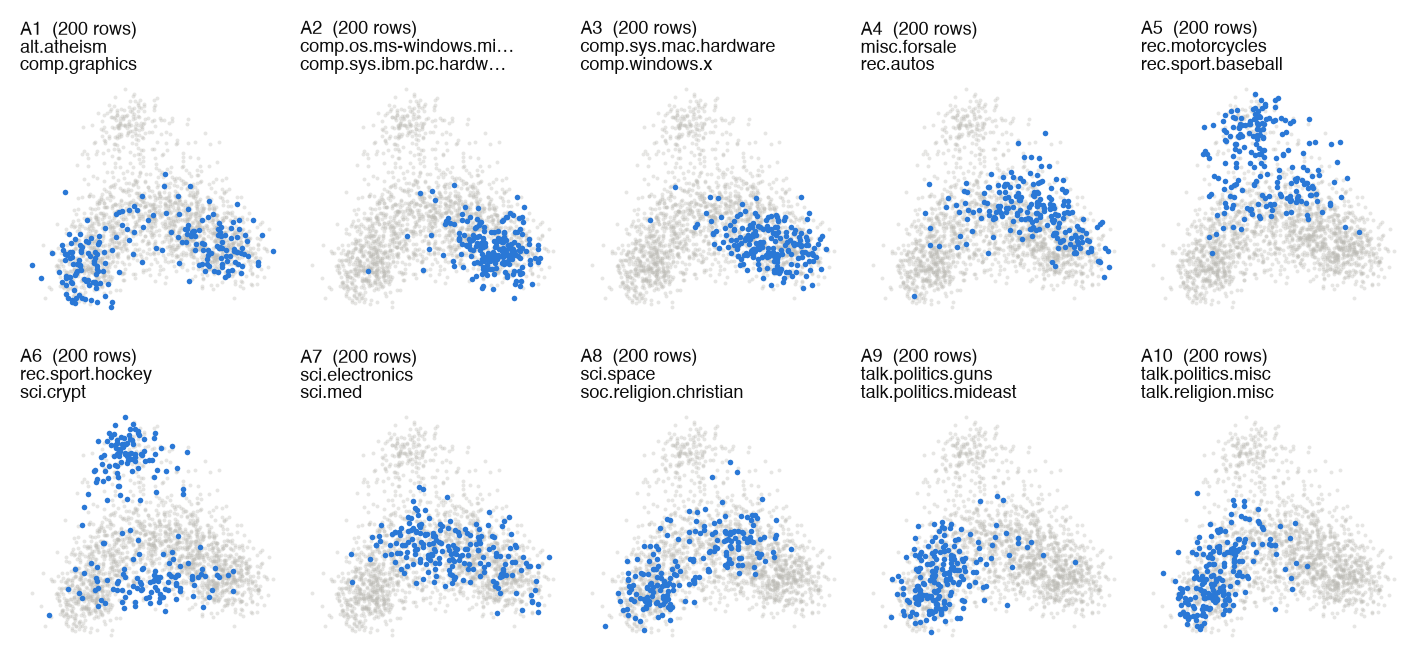
\includegraphics[width=\linewidth]{fig2_per_worker_clusters.png}
  \caption{The same projection as Figure~\ref{fig:projection}, drawn once per edge worker: that
    worker's rows in blue, all other rows in grey. Titles give the worker, the number of its rows that
    reached B, and its two newsgroups.}
  \label{fig:clusters}
\end{figure}

Each panel of Figure~\ref{fig:clusters} shows one node's data arriving at B in its own part of the
plot (sometimes two parts, one per newsgroup, e.g.\ A5: motorcycles vs.\ baseball), distinct from
most other workers. Workers whose topics are related overlap, as expected: A2 and A3 both hold
computer groups, A9 and A10 both hold politics groups, and A8 and A10 share a religion group (these
are also the three most similar pairs of worker centroids in the full \dims-dimensional space).
Workers with unrelated topics (e.g.\ A4: for-sale and cars vs.\ A8: space and religion) occupy
different areas. This is what one would expect from meaningful embeddings, and it is visible after
transport: all \nWorkers{} streams were merged by NebulaStream at~B, yet the structure of every node's
data is preserved and every node delivered all \rowsPerWorker{} of its rows.

\section{Conclusion}

The demo shows that NebulaStream can carry embeddings from \nWorkers{} edge nodes to one node: all
\rowsTotal{} rows arrived complete and unchanged, B computed on them inside NebulaStream, and the
result is meaningful (Figure~\ref{fig:projection}: topic recognised by similarity;
Figure~\ref{fig:clusters}: each node's data keeps its own structure). Sending embeddings instead of
the raw posts needed \ratio$\times$ fewer bytes.

\paragraph{Limits of this first version.}
Embeddings were computed offline, not on the edge nodes, so the cost of computing them at the edge is
not yet included. The byte comparison uses uncompressed text and payload bytes, not NebulaStream's
wire format. A single SQL dot product compiles only up to 64 dimensions in this NebulaStream build
(embeddings themselves travel fine up to 256). There is no aggregation yet; intermediate aggregating
nodes are the next step toward hierarchical topologies.

\end{document}
